% Chapter 2

\chapter{Resultados} % Main chapter title

\label{Chap:Res} % For referencing the chapter elsewhere, use \ref{Chapter2} 

\section{Introducción}

En este capítulo se presentarán los procedimientos requeridos para llevar a cabo el experimento descrito en el capítulo anterior, y se expondrán los resultados obtenidos de realizar las mediciones. Posteriormente, se mostrarán gráficas de los datos obtenidos con una explicación de sus componentes y su respectiva interpretación. \\

\section{Dibujo del plano}

Para el trazo de la figura, que será de 15 metros por lado, se utilizaron dos varas unidas por una fracción de rafia como las de la figura~\ref{fig:HerTraz}, utilizados para el trazado de las circunferencias necesarias.\\

\begin{figure}[H]
\centering
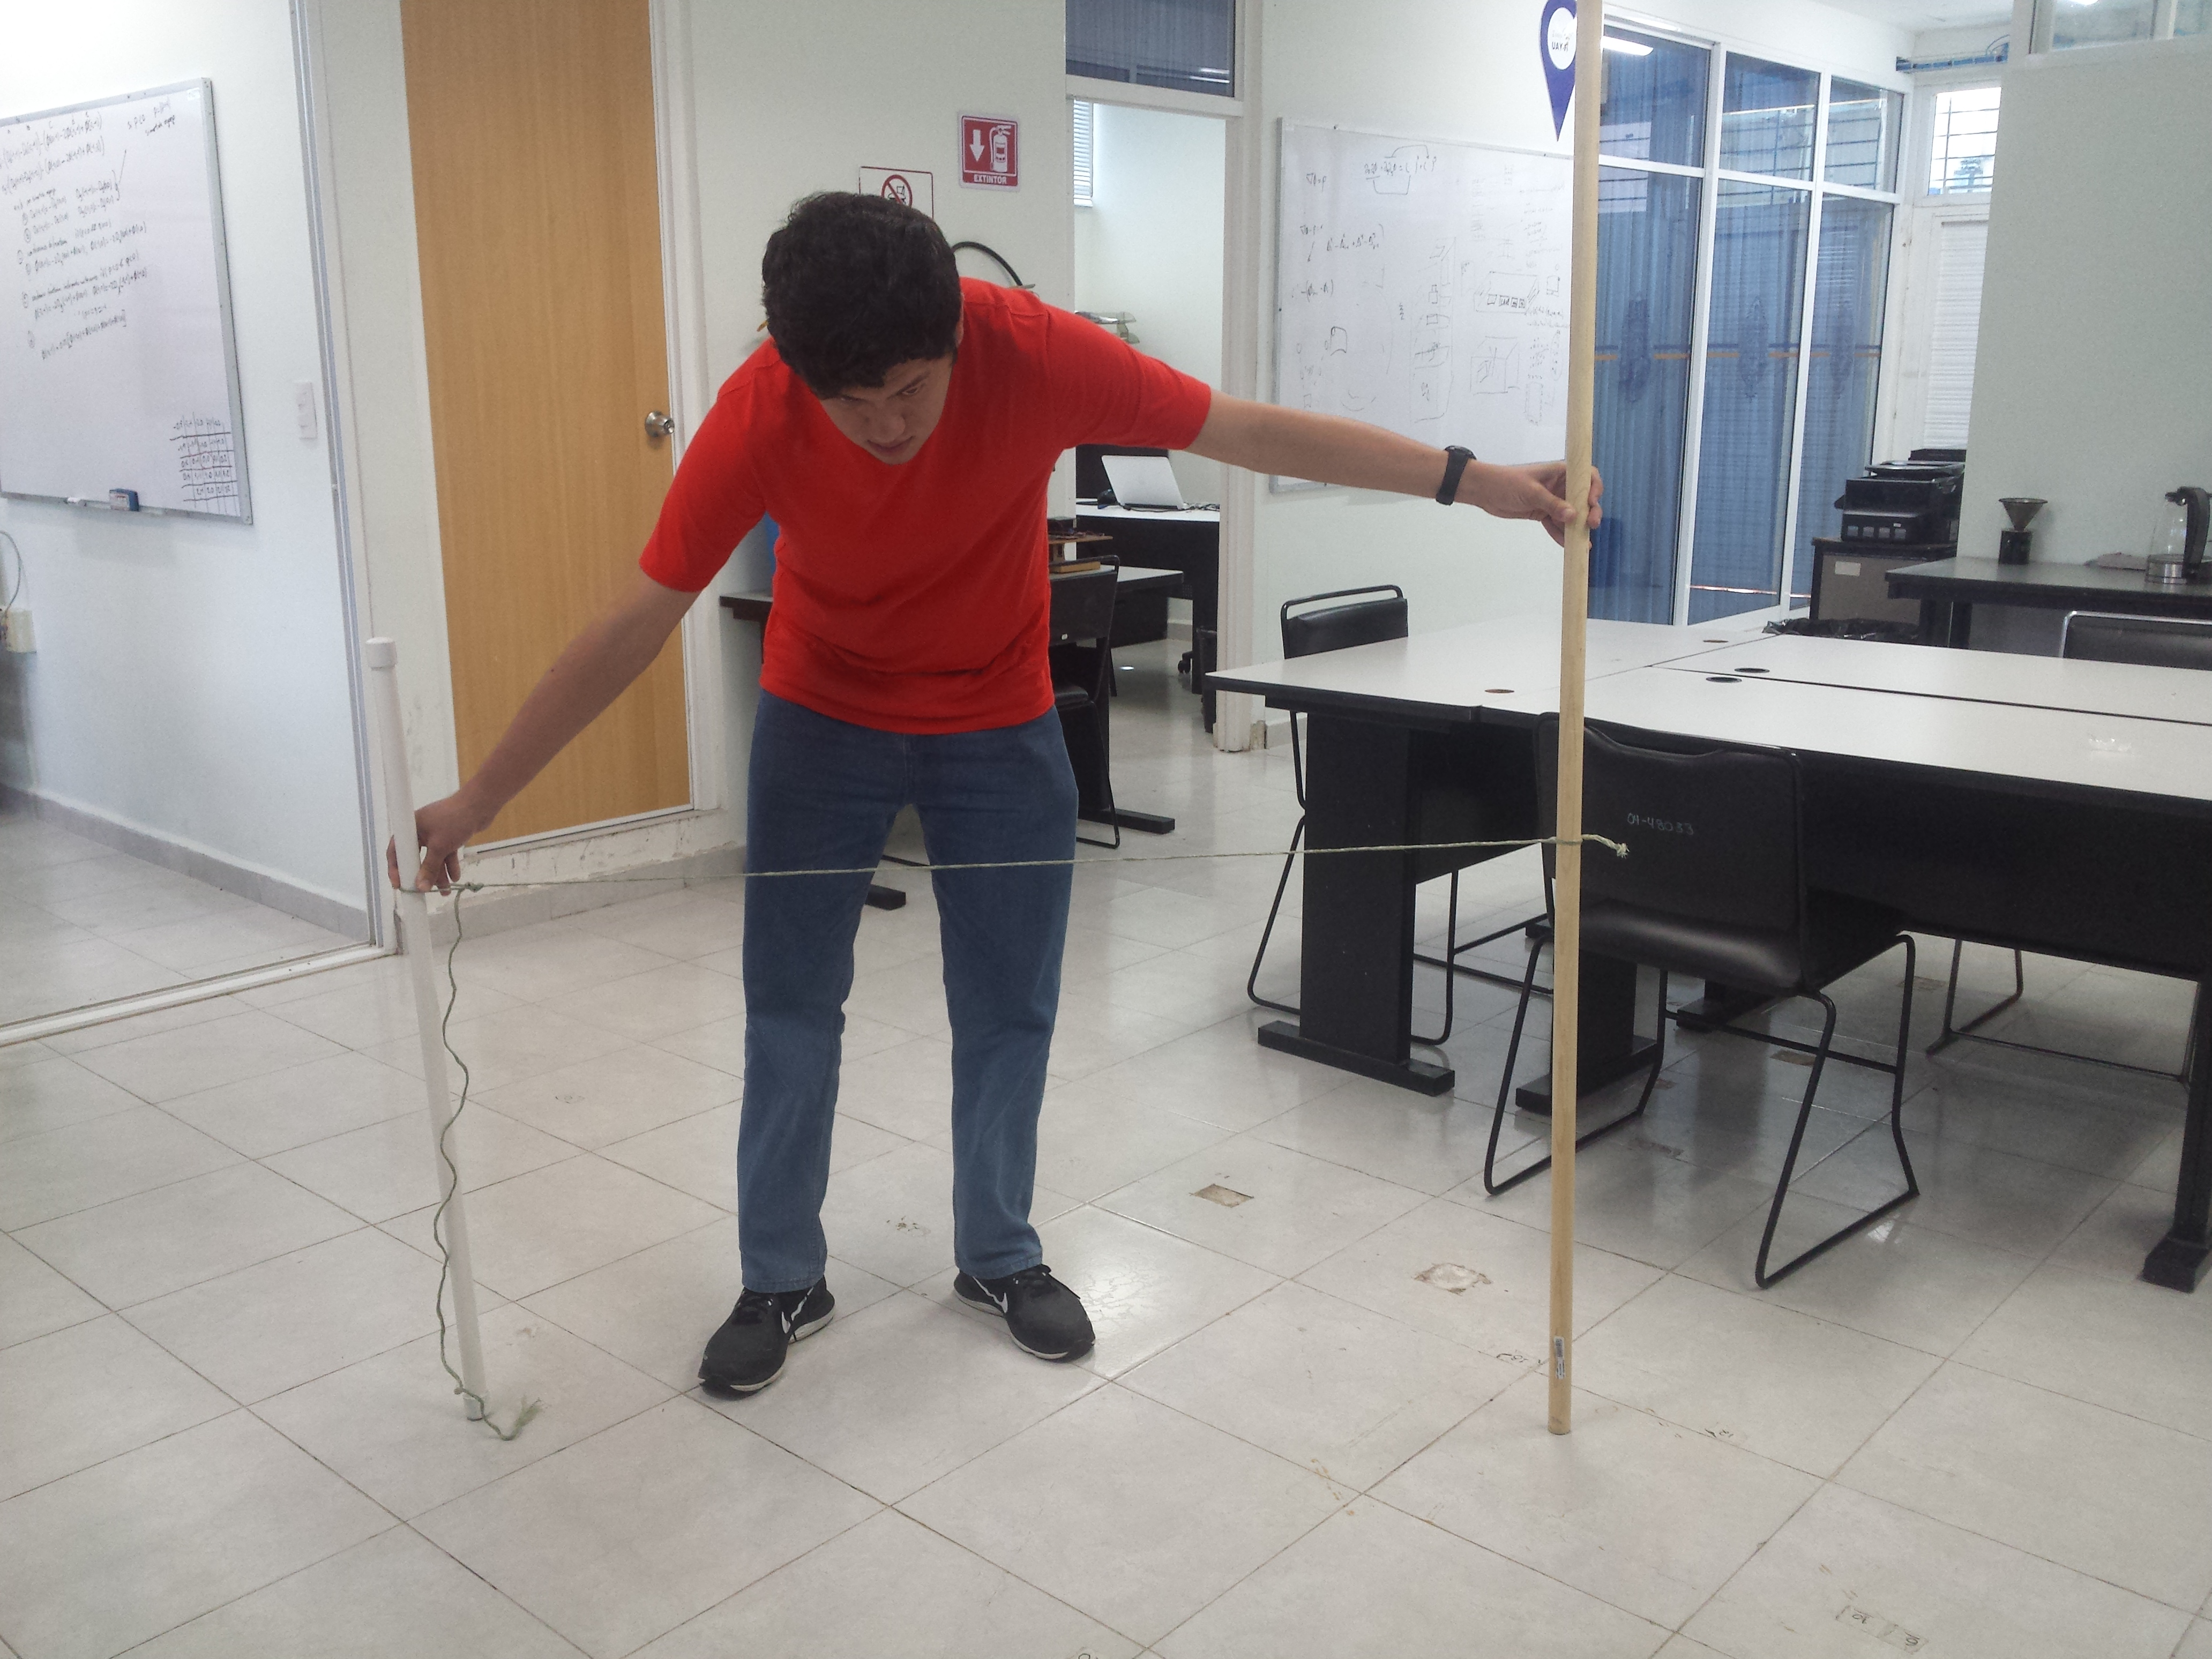
\includegraphics[width=0.95\textwidth]{Figures/Herr}
\caption[Herramientas de trazado.]{Herramientas de trazado.}
\label{fig:HerTraz}
\end{figure}

Para garantizar que se trace una línea recta en cada uno de los lados de la figura, se utilizó una cuerda de nailon de 17 metros de longitud, que una vez tensa, permitió realizar las marcas equidistantes cada 3 metros con un flexómetro, signos en el suelo como los de la figura~\ref{fig:MarEq}.

\begin{figure}[H]
\centering
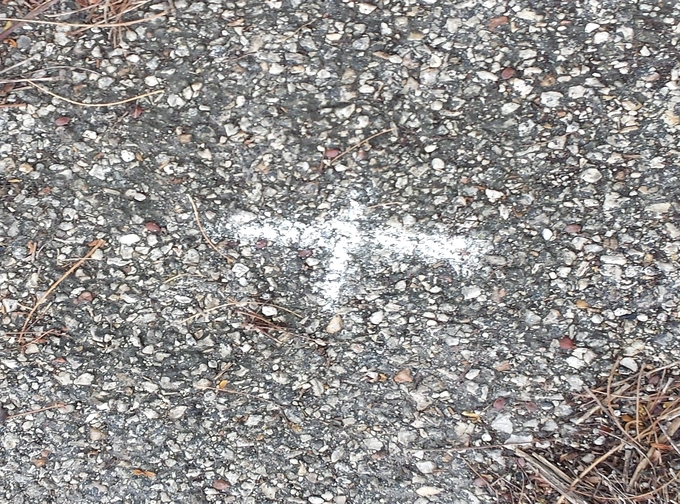
\includegraphics[width=0.95\textwidth]{Figures/Equid}
\caption[Marcas equidistantes en el suelo.]{Marcas equidistantes en el suelo.}
\label{fig:MarEq}
\end{figure}

\section{Mediciones}
Una vez finalizada la separacíon por segmentos de cada lado de la figura, y de ser configuradas ambas estaciones, se procedió a realizar las mediciones de las coordenadas en los puntos. Se decidió tomar muestras tanto en el modo Real-Time Kinematics como con el modo de un solo GPS sin retroalimentación de una estación base para comparar resultados. En ambos modos, se recorrió el trazado de la figura en dos ocasiones con la antena, en dos sentidos diferentes, llegando a obtener dos mediciones de coordenadas por punto en cada modo de funcionamiento.\\

\begin{figure}[H]
\centering
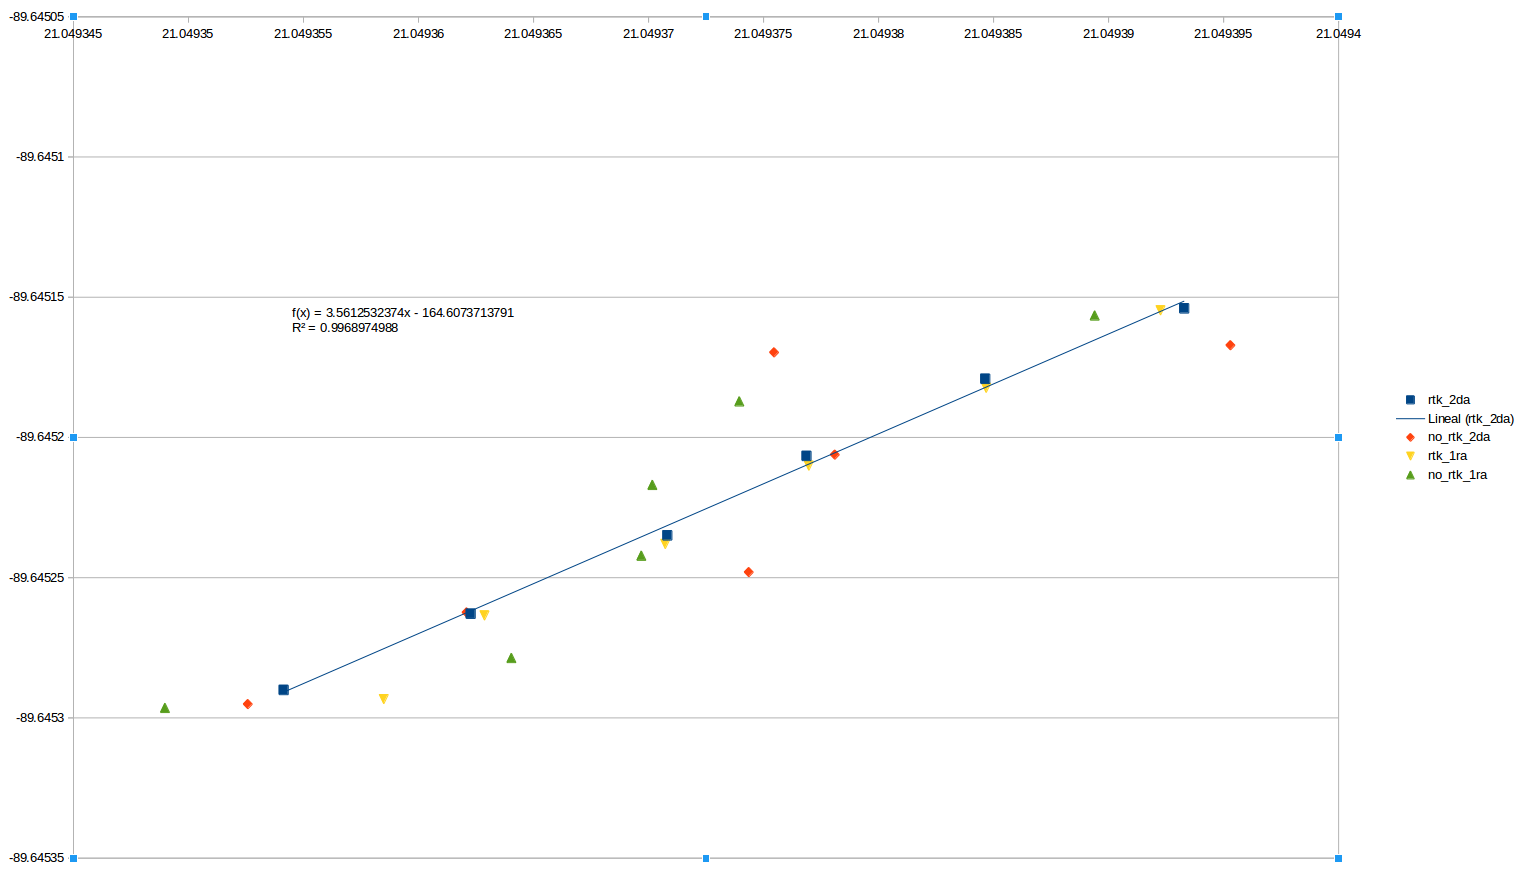
\includegraphics[width=0.95\textwidth]{Figures/Dispers}
\caption[Diagrama de dispersión de datos en las marcas del lado sur de la figura.]{Diagrama de dispersión de datos en las marcas del lado sur de la figura.}
\label{fig:Disp}
\end{figure}

En la figura~\ref{fig:Disp} se comparan las mediciones realizadas en las marcas del lado sur de la figura, mediante una regresión lineal. Los cuadrados azules marcan la segunda vuelta realizada en el modo Real-Time Kinematics. Los triángulos amarillos marcan las muestras de la primera vuelta en el mismo modo. El rombo rojo y el triángulo verde marcan el mismo orden pero del modo con un solo GPS sin retroalimentación de posicionamiento.\\

Las muestras realizadas en el modo Real-Time Kinematics muestran, en su segunda vuelta, un mayor ajuste a la línea recta de la figura, donde el valor del coeficiente de correlación múltiple $R^{2} \approx 0.997$\footnotemark sugiere un alto ajuste a una línea recta. En la primera vuelta, marcada con triángulos amarillos, se puede observar la misma tendencia pero con un menor ajuste. El resto de puntos son en un modo sin Real-Time Kinematics y se puede observar que el ajuste a una línea recta es mucho menor que el modo RTK, llegando a tener variaciones bastante considerables respecto a dicho método.\\

\footnotetext{El valor de $R^{2}$ varía de 0 a 1. Mientras más cerca esté su valor de la unidad, se sugiere una correlación más alta a la recta en este caso.}

En el modo Real-Time Kinematics, en cada muestra, existe un valor denominado \textit{\textbf{ratio}} que indica la calidad de la señal de los satélites y de las mediciones del GPS en el \textit{rover} de forma proporcional. En otras palabras, mientras más alto sea el valor de ratio, mucha mejor será la corrección de la señal de GPS. En la figura~\ref{fig:Ratio} se observa cómo en las primeras muestras, el valor del ratio oscilaba en valores bajos (se consideran valores bajos aquellos que están debajo de 3). Conforme el tiempo avanzaba, se captaban más satélites y, como consecuencia, el valor del ratio ascendió a valores altos. Este comportamiento se ajusta a la gráfica de dispersión en la figura~\ref{fig:Disp}, que muestra que la primera vuelta, denotada con un triángulo amarillo, estuvo algo más separada de la recta que el resto de muestras de su misma rutina.

\begin{figure}[H]
\centering
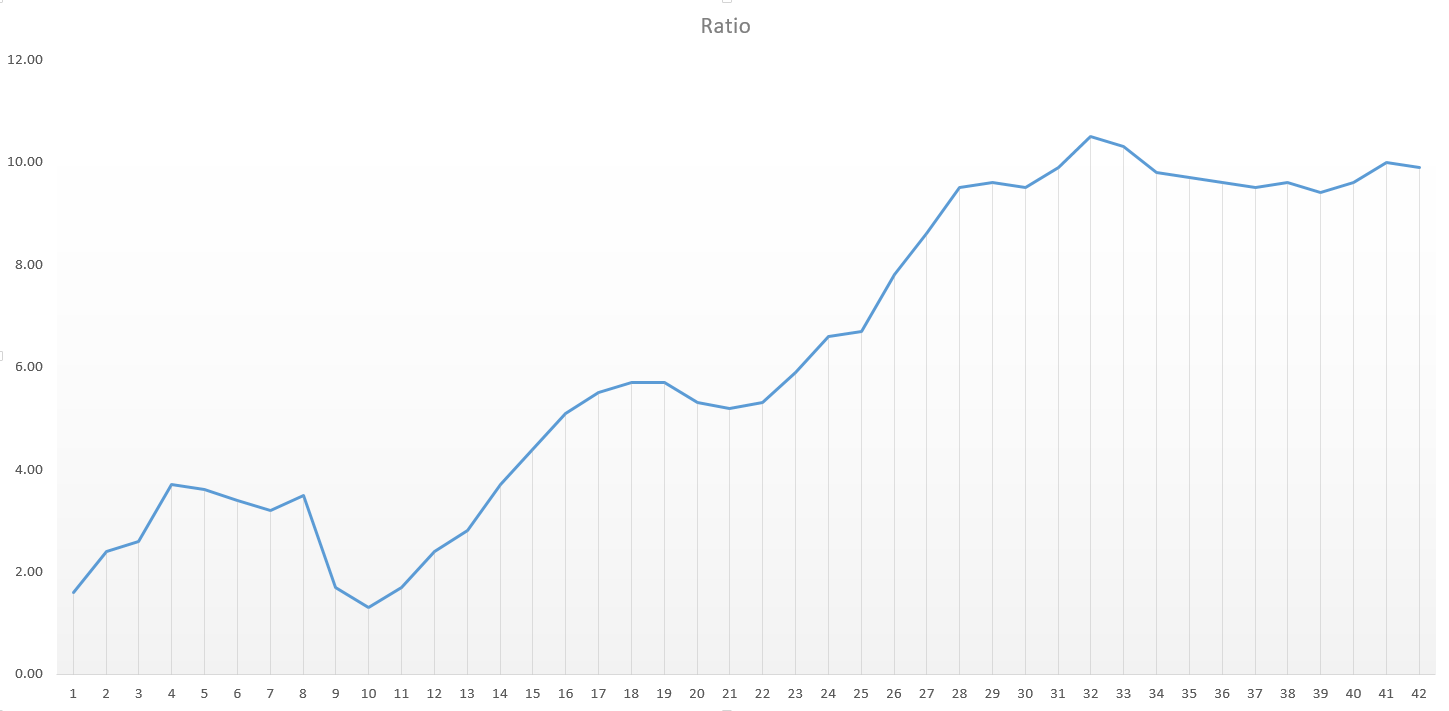
\includegraphics[width=0.95\textwidth]{Figures/Ratio}
\caption[Gráfica del ratio.]{Gráfica del ratio.}
\label{fig:Ratio}
\end{figure}

Finalmente, las coordenadas obtenidas durante la rutina se muestran en el mapa en las figuras~\ref{fig:NoRtkRes}~y~\ref{fig:RtkRes}, siendo la primera la solución RTK y la segunda la solución sin retroalimentación.

\begin{figure}[H]
\centering
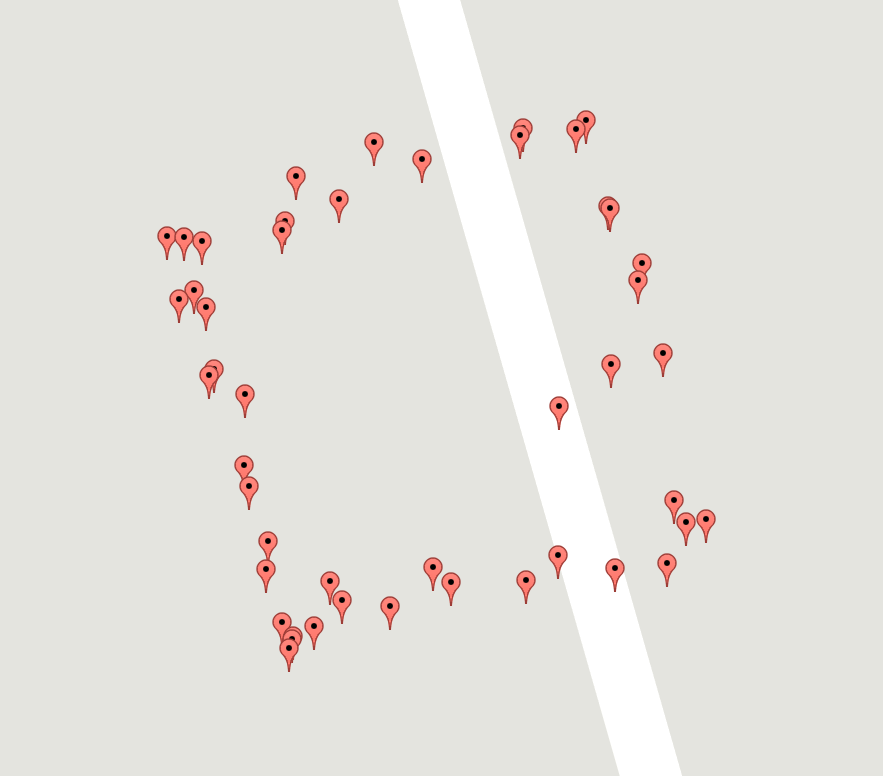
\includegraphics[width=0.95\textwidth]{Figures/NoRtkRes}
\caption[Muestras sin Real-Time Kinematics.]{Muestras sin Real-Time Kinematics.}
\label{fig:NoRtkRes}
\end{figure}

\begin{figure}[H]
\centering
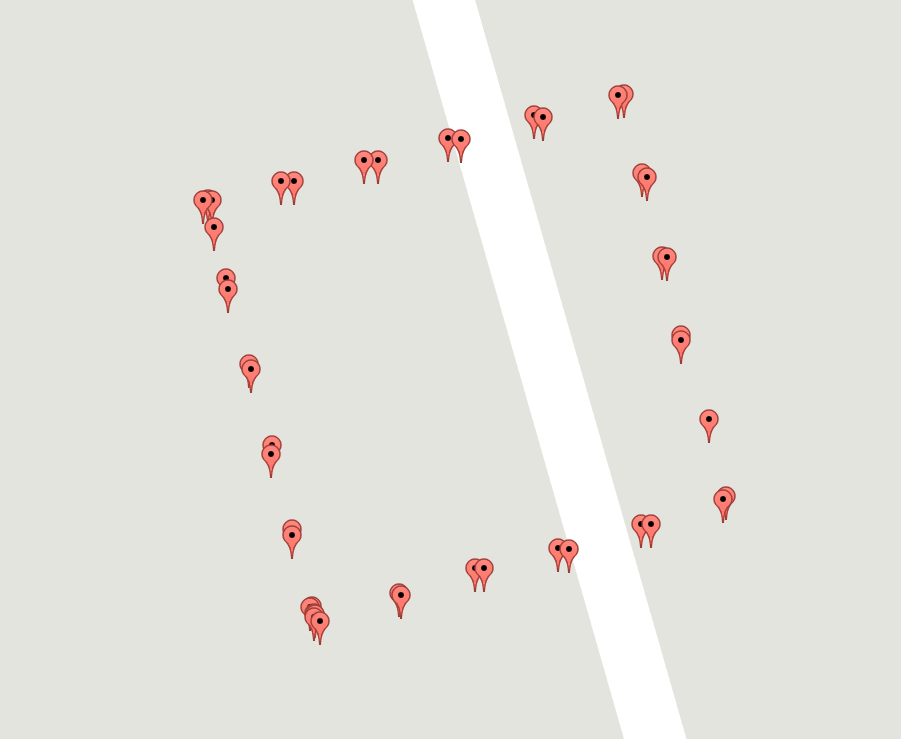
\includegraphics[width=0.95\textwidth]{Figures/RtkRes}
\caption[Muestras con Real-Time Kinematics.]{Muestras \textbf{con Real-Time Kinematics}.}
\label{fig:RtkRes}
\end{figure}

Nótese cómo en la solución sin retroalimentación (figura~\ref{fig:NoRtkRes}) se muestran variaciones muy altas en la línea recta y las muestras se ven afectadas notoriamente en el lado este de la figura. Por otro lado, en la solución con RTK se muestra un mucho mejor ajuste a los puntos marcados y se observa un mejor acoplamiento a la forma de la figura.

\section{Conclusión}
Tras el análisis de los resultados, se determinó que la solución con Real-Time Kinematics ayuda a mantener la estabilidad de las mediciones de GPS, pudiendo determinar mejor la posición de puntos durante una rutina previamente estructurada.